The Liaison System is created to assure that the correct data collected from a microcontrollers is received correctly by the end user.
To achieve this, the system uses four equal but distinct microcontrollers, an internal voting system to assure that if any of the microcontrollers
disagree, it is marked as malfunctioning and is no longer allowed to send output. The output sent from the Liaison is extended with a system status
code that tells the end user if any of the microcontrollers are damaged, and the signal is also enhanced with an error correcting code such that
we can be more certain that the signal is not distorted on its way to the reciever.

\begin{figure}
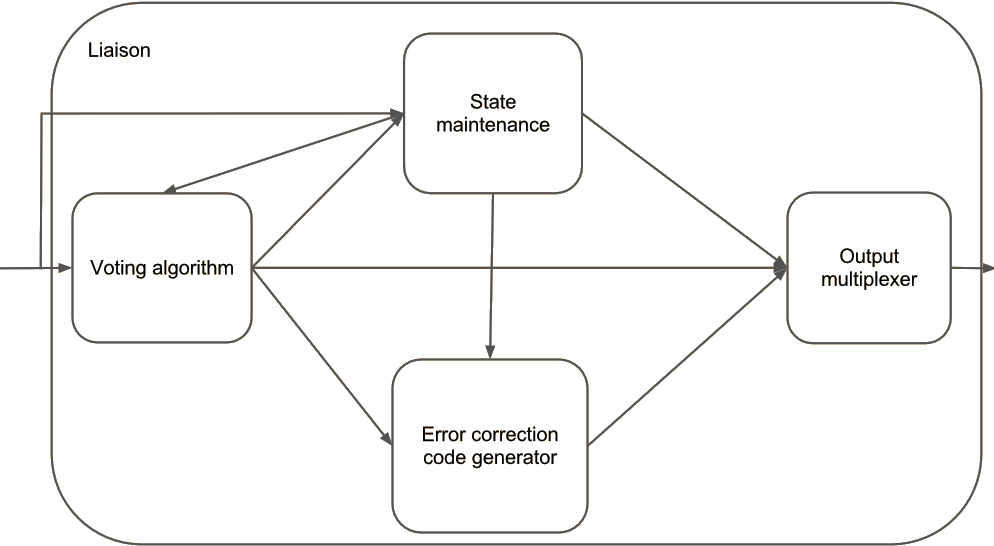
\includegraphics[width=15cm]{design/fig_overview}
\caption{Modules overview}
\label{fig:overview}
\end{figure}

As we can see from \autoref{fig:overview}, the internals of the Liaison can be modeled as four different pieces of hardware, each providing a
nessesary service to the system.

\subsection{Voting algorithm}
\subsection{State maintainance}
\subsection{Error Correcting Code Generator}
\subsection{Output mulitplexer}
